\documentclass[../main.tex]{subfiles}
\begin{document}

\section{Verfahren}

\subsection{Datenerfassung}
Ziel ist ein digitales Abbild von einem realen Objekt zu erstellen.
Als Grundlage für dieses Abbild arbeite, ich in diesem Fall mit Pointclouds 
die mithilfe eines Laserscanners aufgenommen wurden. Auch andere Möglichkeiten
Pointclouds zu erhalten sind denkbar und sollten mit dem Verfahren 
kompatibel sein.

\subsection{Versuchsaufbau}

\begin{wrapfigure}{r}{0.6\textwidth}
    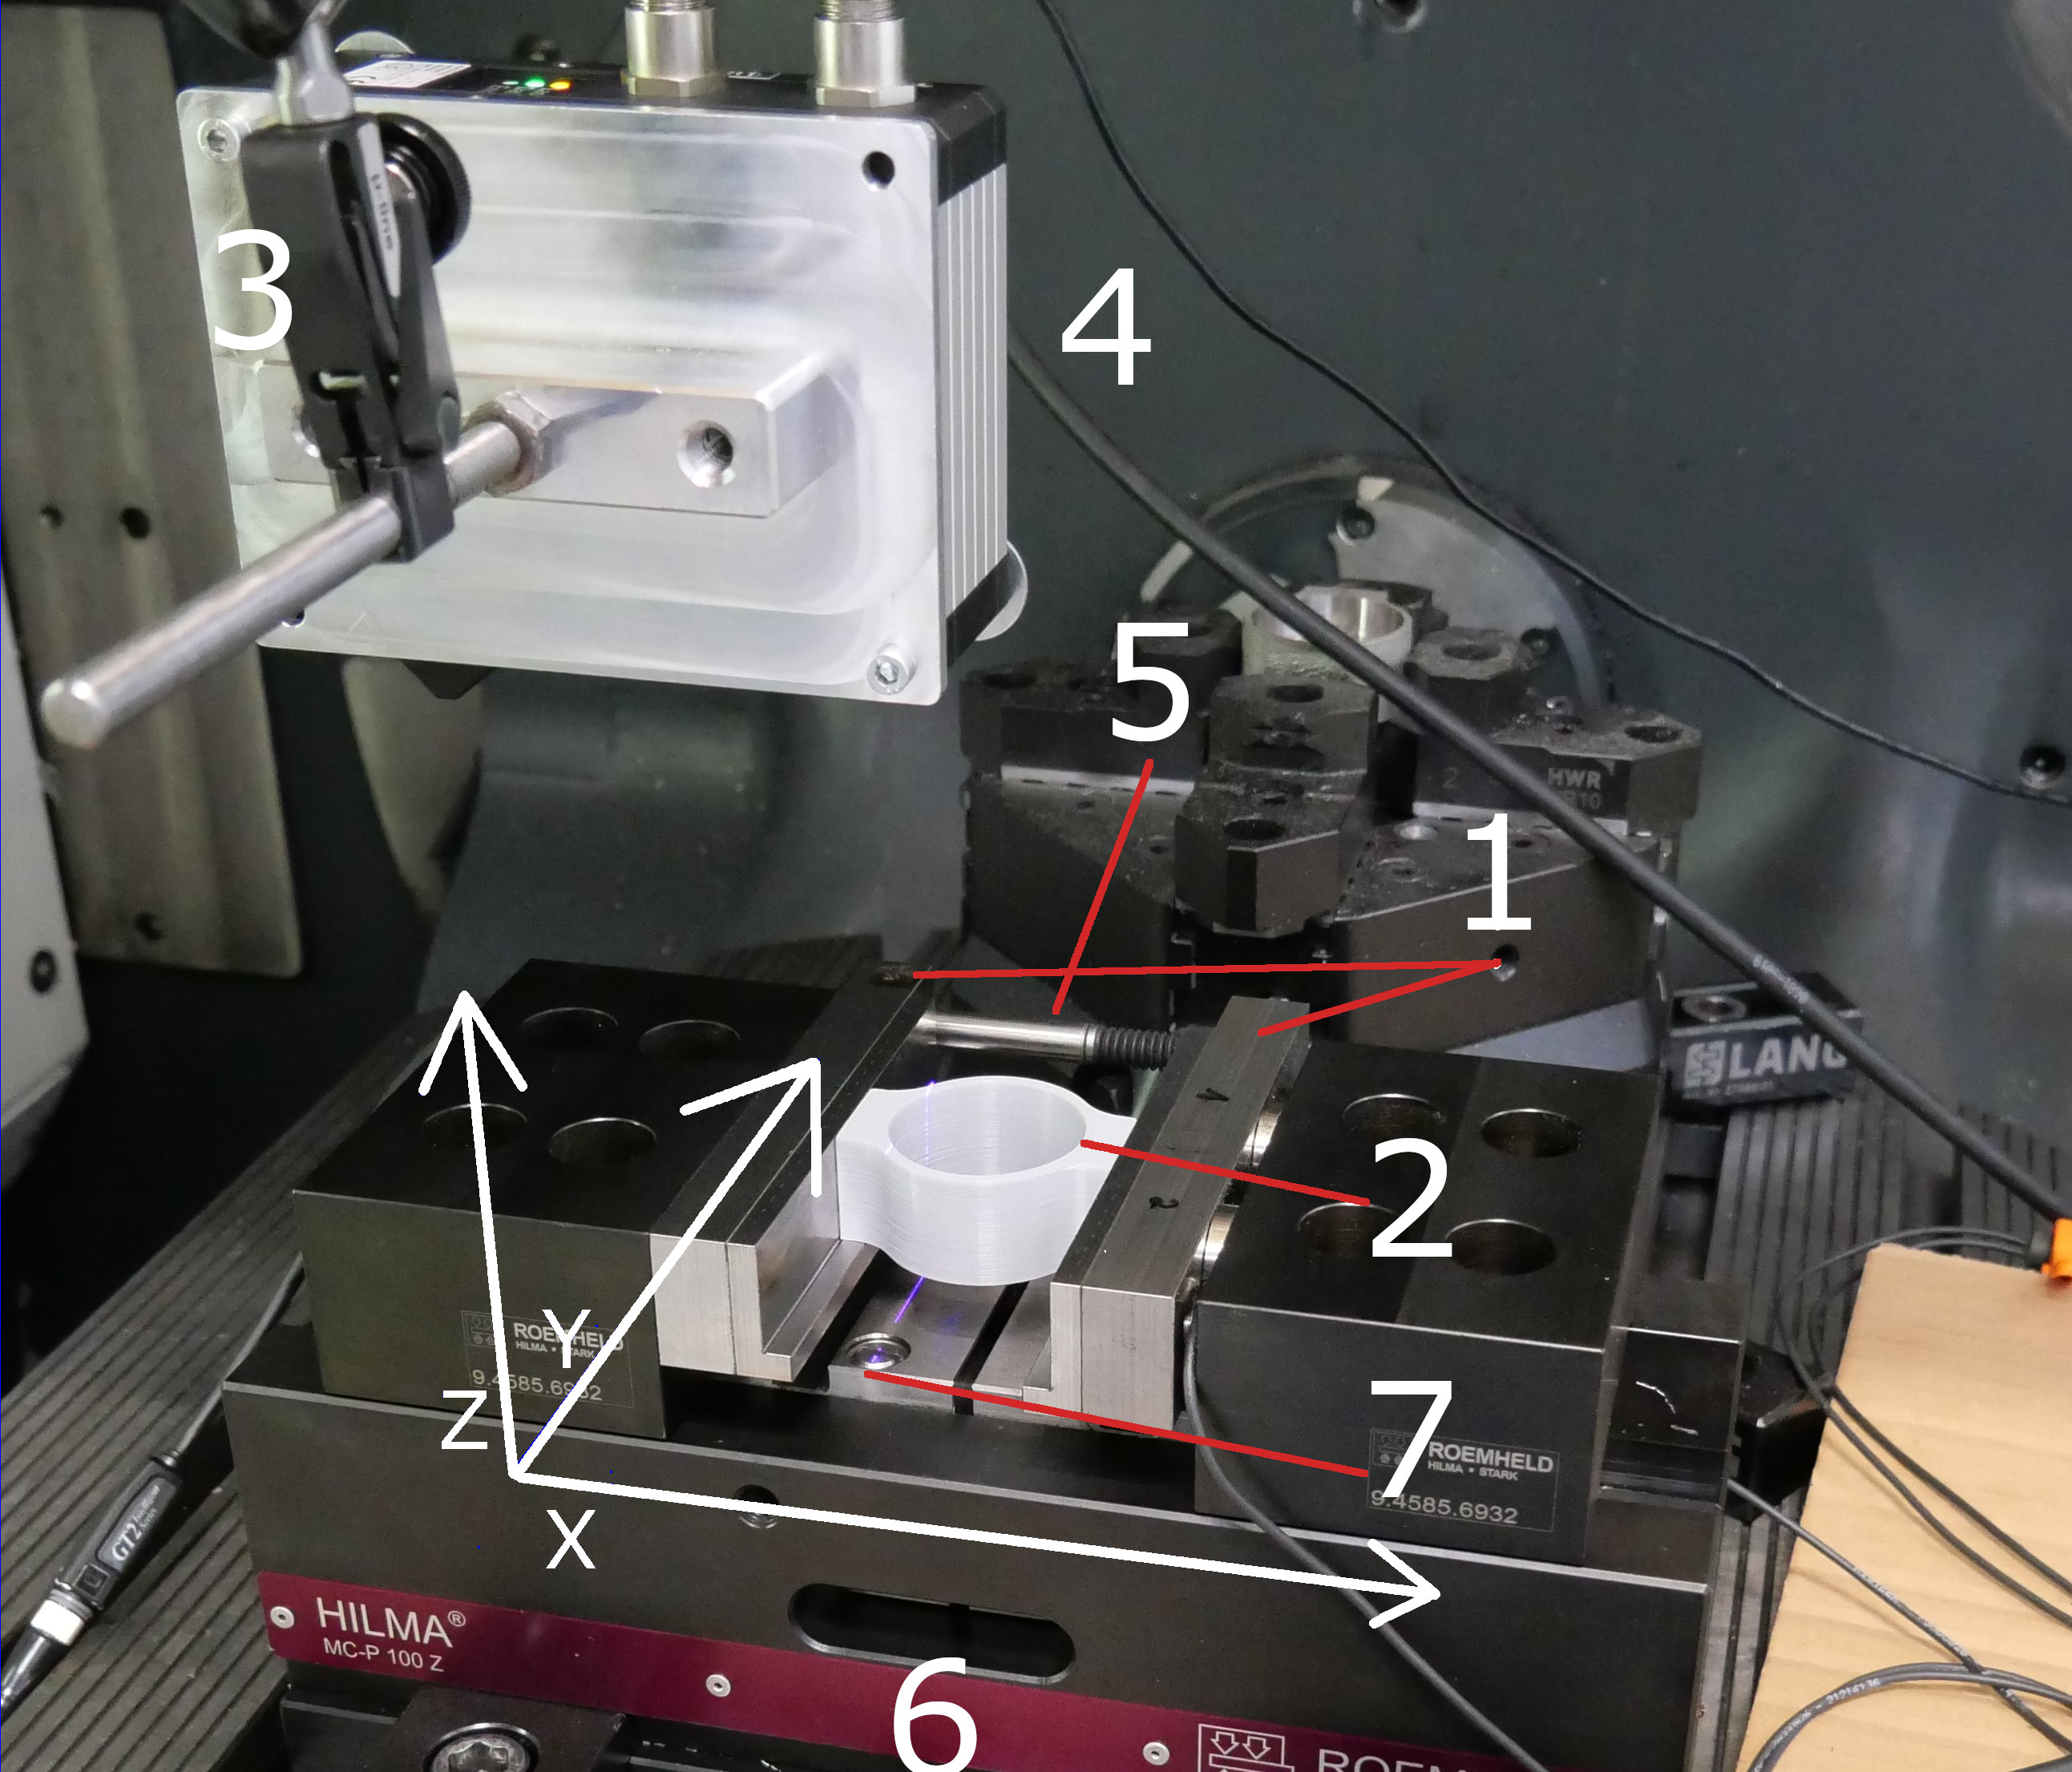
\includegraphics[width=0.6\textwidth]{images/versuchsaufbau_foto.png.JPG}
    \caption{Versuchsaufbau}
    \label{fig:versuchsaufbau}
\end{wrapfigure}

In Abbildung \ref{fig:versuchsaufbau} ist der Versuchsaufbau zur Datenerfassung 
zu sehen. Alle wichtigen Bestandteile sind nummeriert. Es folgt eine kurze Benennung
aller vorhandenen und notwendigen Teile:\\
1: Schraubstock Backen\\
2: Demonstratorbauteil\\
3: Scannerhalterung\\
4: Scanner LLT 30x0-25\\
5: Verschiebungsmesser\\
6: Laserlinie (Lila)\\
7: Schraubstock mit Kraftmesser\\
X: x-Achse\\
Y: y-Achse\\
Z: z-Achse\\

Der Scanner ist an dem Werkzeugkopf einer CNC-Fräse befestigt und wird 
in Richtung der X und Y Achse verschoben. So kann von dem kompletten Bauteil eine 
Pointcloud aufgenommen werden.

\subsubsection{Geschwindigkeit}
Der Parameter `Geschwindigkeit` muss der realen Vorlaufgeschwindigkeit des Scanners
entsprechen um eine korrekte und akkurate Pointcloud zu erhalten. Ist die 
Messgeschwindigkeit kleiner als die Bewegung des Scanners werden Profile doppelt 
aufgenommen, ist sie zu hoch werden Profile übersprungen und das Bauteil wirkt in 
der resultierende Pointcloud in X-Richtung gestreckt.

\begin{wrapfigure}{l}{0.25\textwidth}
    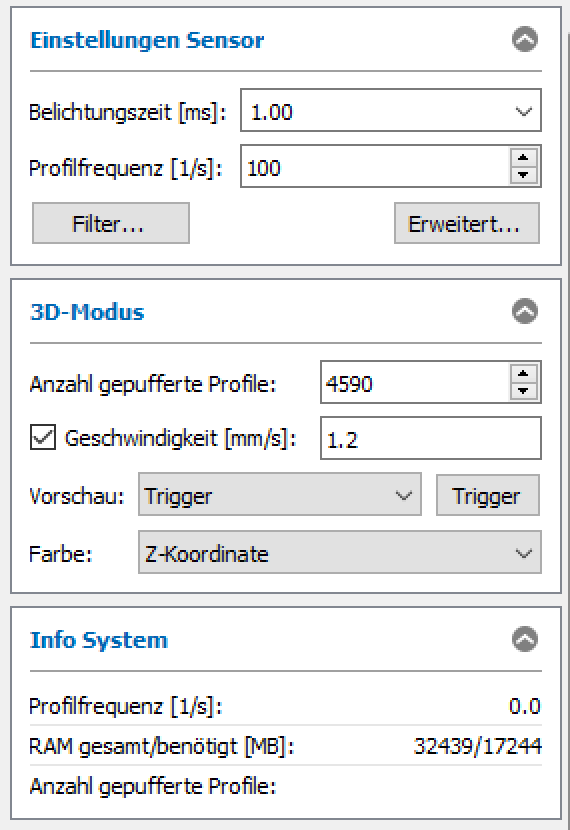
\includegraphics[width=0.25\textwidth]{images/Parameter_Scan.png}
    \caption{Scanparameter}
    \label{fig:scanparameter}
\end{wrapfigure}

\subsubsection{Limitierungen der Achsen:}

Die gesamte Länge des Objekts kann also erfasst werden, indem Scanner 
beziehungsweise Werkzeugkopf in X-Richtung verschoben wird. Mit dem Start der 
Bewegung muss auch die Aufzeichnung der Scannerdaten beginnen. In unserem Fall wurde
die Datenerfassung manuell per Hand im richtigen Zeitpunkt über die Software 
'SCANControl' von micro-epsilon gestartet. 
Eine mögliche Verbesserung ist es, diesen Vorgang zu automatisieren, indem der 
Scanner automatisch mit dem Start der Bewegung getriggert wird und die Aufzeichnung
startet. Die Länge der Aufzeichnung wird auch über die Software eingestellt. 
In Abbildung \ref{fig:scanparameter} sind die korrekten Parameter für das 
Demonstratorbauteil zu sehen. Über den Parameter 'Anzahl gepufferte Profile' kann 
die Länge der Aufzeichnung eingestellt werden. Limitiert wird dieser Parameter 
durch den verfügbaren Speicher auf dem Zielsystem. Es sollte auch darauf geachtet 
werden das der Scanner mindestens genauso lange bewegt wird wie Aufzeichnung läuft, 
ist dies nicht der Fall entsteht eine Pointcloud die einmal größer als notwendig ist, 
und außerdem am Ende der x-Achse nur wiederholende Profile beinhalten. 
Die y-Achse der Pointcloud wird durch den eingesetzten Scanner limitiert. 

\begin{wrapfigure}{r}{0.2\textwidth}
    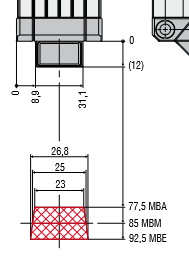
\includegraphics[width=0.2\textwidth]{images/Scanner.PNG}
    \caption{Scanner}
    \label{fig:scanner}
\end{wrapfigure}

Der Scanner hat Abhängig vom Modell und der angebrachten Höhe eine fixe Länge die 
er aufnehmen kann. In unserem Fall wurde der Scanner 'LLT 30x0-25' verwendet der 
eine mittleren Messbreite von 25 mm bietet. 
(Siehe Abbildung \ref{fig:scanner} \cite{MESSTECHNIK_2020}) 
Bauteile mit einer größeren Länge in Y-Richtung können also nicht in einer Pointcloud
erfasst werden. Damit eine Digitalisierung von größeren Objekten erfolgen kann, müssen
also mehrere Scans durchgeführt, und später zusammengefügt werden. Zwischen den 
Scanvorgängen muss der Scanner in Y-Richtung verschoben werden.
Die Länge der Verschiebung sollte 
kleiner als die Scannerbreite sein, damit eine Überlappung entsteht, die 
genutzt werden kann, um die Pointclouds wieder zusammenzufügen. Die Verschiebung kann 
beliebig klein gewählt werden, jedoch steigt der Arbeitsaufwand und die Dateigröße mit 
jeder zusätzlichen Pointcloud, während das Ergebnis sich nicht verbessert.
So können Pointclouds aufgenommen werden die dann in dem zu entwickelnde Verfahren
wieder zu einem digitalen Abbild zusammengefügt werden. Ist dieser Prozess erfolgreich
erhält, man eine Pointcloud der Oberfläche des Objekts. 
In Abbildung \ref{fig:pointcloud_big} ist eine Pointcloud von dem Demonstratorbauteil
zu sehen, in Abbildung \ref{fig:pointcloud_small} eine Nahaufnahme des mittleren Teils
derselben Pointcloud in der die einzelnen Punkte sichtbar sind. Hier sieht man wie
die Pointcloud aufgebaut ist. Dazu aber später noch etwas mehr.

\begin{figure}[h]
    \centering
    \begin{minipage}{0.45\textwidth}
        \centering
        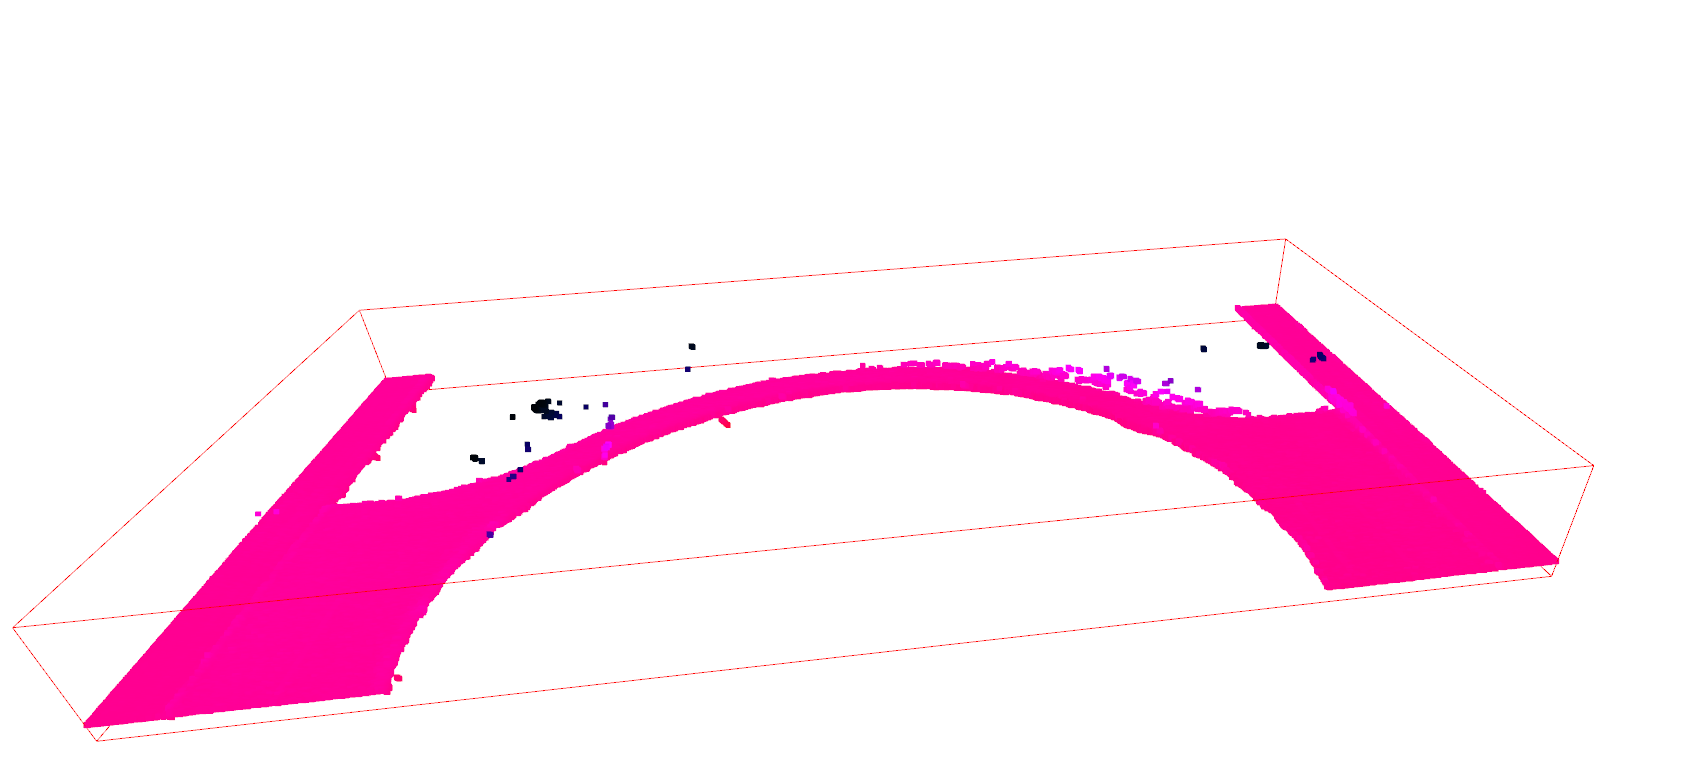
\includegraphics[width=0.9\textwidth]{images/pointcloud_big.PNG} % first figure itself
        \caption{Pointcloud}
        \label{fig:pointcloud_big}
    \end{minipage}\hfill
    \begin{minipage}{0.45\textwidth}
        \centering
        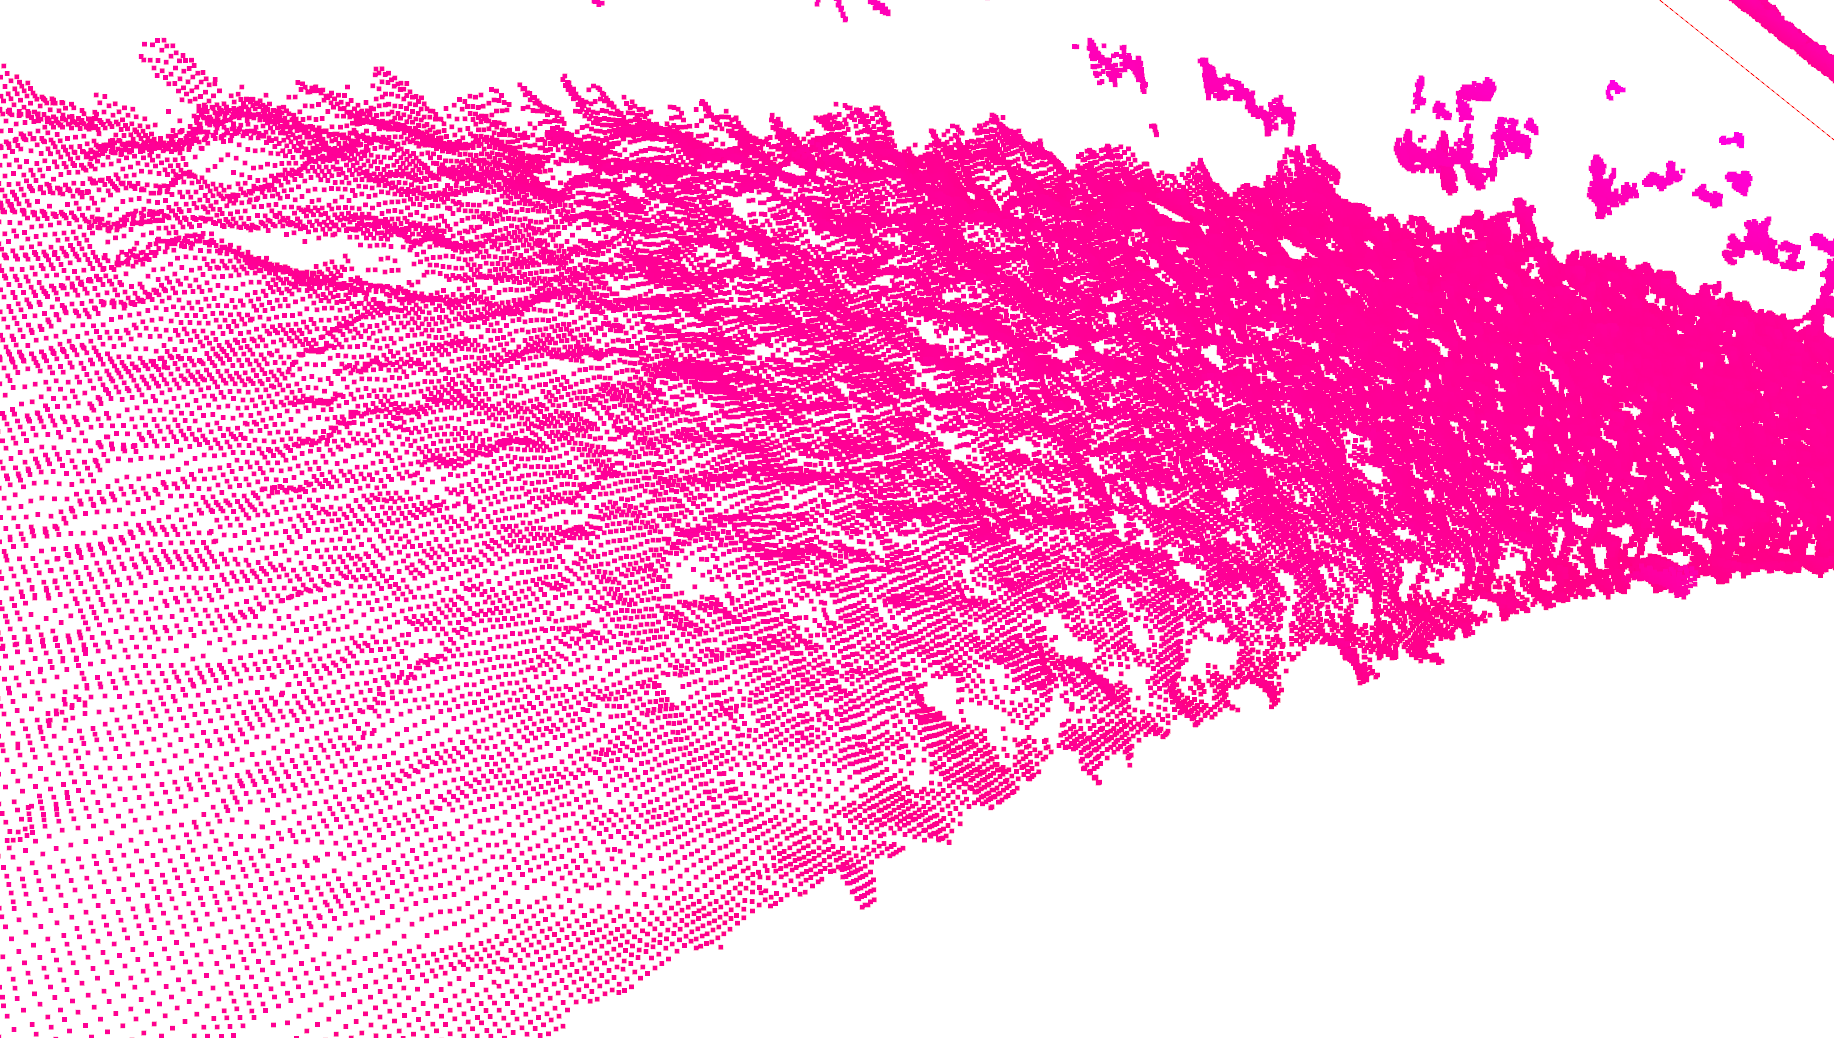
\includegraphics[width=0.9\textwidth]{images/pointcloud_small.PNG} % second figure itself
        \caption{Nahaufnahme Pointcloud}
        \label{fig:pointcloud_small}
    \end{minipage}
\end{figure}

\needspace{0.4\textwidth}
\begin{wrapfigure}{r}{0.4\textwidth}
    \includegraphics[width=0.4\textwidth]{images/taster.JPG}
    \caption{Taster}
    \label{fig:taster}
\end{wrapfigure}

\subsubsection{Zusätzliche Messinstrumente}

Zusätzlich zu dem Scanner werden noch mit weiteren Elementen Daten erfasst.
In Abbildung \ref{fig:versuchsaufbau} unter der Nummer 5 ist ein mechanischer 
Verschiebungsmesser zu sehen. Dieser misst die Verschiebung der Backen des 
Schraubstocks. Der Schraubstock misst zusätzlich mit viel Kraft die Backen 
aufeinander pressen. Damit die Scanner-Ergebnisse überprüft werden können 
wird die Bauteilgeometrie zusätzlich nach dem Scanvorgang noch mit einem Taster
abgetastet. Hierfür wird der Werkzeugkopf gewechselt und der Scanner entfernt.
Dann wird der Taster in die CNC-Maschine eingesetzt und das Bauteil abgetastet.
In Abbildung \ref{fig:taster} ist das Tasterwerkzeug zu sehen. Die rote Kugel 
am Ende des Tasters erkennt, sobald eine Berührung zu dem Bauteil erfolgt ist 
und benachrichtigt den Steuerungsrechner. Dieser speichert die aktuelle Position 
dann in einer Protokolldatei. 

Bevor ich mich aber mit dem 2. Schritt des Verfahrens beschäftigen möchte ich auf die 
Datenstruktur von Pointclouds eingehen. Wie der Name schon sagt bestehende
Pointclouds aus Punkten. In unserem Fall ca. 3 Millionen für eine einzelne
Bewegung in X-Richtung. In jedem Punkt sind mindestens 3 Koordinaten gespeichert, 
eine X und Y Koordinate relativ zu Ursprung der Pointcloud und eine Z Koordinate 
in der die Höhe gespeichert wird. Der Ursprung der Pointcloud liegt in der Mitte 
der x-Achse, also genau da wo der Scanner verläuft.
Zusätzlich ist für jeden Punkt auch noch eine Farbe als RGB-Farbwert
(3 Werte von 0 bis 255) gespeichert. Die Farbe wird relativ zu der Höhe
berechnet. Punkte bekommen einen Farbwert zugewiesen je nachdem wie nah 
sie an dem Minimum oder Maximum der Z-Koordinate sind. 
In \ref{fig:pointclouds} ist die komplette Pointcloud eines Demonstratorbauteils 
zu sehen, zusammen mit einer BoundingBox, durch diese werden die Randpunkte
der Pointcloud visuell dargestellt. Man sieht außerdem das unten liegende Punkte
hell und weiter oben liegende Punkte dunkler dargestellt werden.
Unterhalb ist eine Nahaufnahme des Mittelstücks des gleichen Bauteils zu sehen. 
Hier sind die einzelnen Punkte sichtbar.

Die Koordinaten sind als Float gespeichert haben keinerlei Bezug zueinander.
Das heißt die X und Y Koordinaten sind nicht zum Beispiel anhand eines Netzes
angelegt, sondern können einen beliebigen Abstand zwischen einander haben. Das
werden wir auch später in der weiteren Bearbeitung der Pointclouds sehen.

Wenn nun also alle Pointclouds für ein Objekt erfasst wurden kann zu dem 2.
Schritt des Verfahrens übergegangen werden. Hier müssen die Daten zusammengefügt 
werden. 
Hierfür existieren in der Literatur schon verschiedene Verfahren, ein 
besonders beliebtes ist der ICP-Algorithmus.
Dieser Algorithmus existiert schon seit dem Beginn der 90er Jahre und ist 
die klassische Methode, wenn es um die Registrierung von Pointclouds und 
anderen Punkt-Sets geht. \cite[]{icp}
Der Algorithmus errechnet eine lokale, optimale Transformation die ein Datenset
dem anderen annähern kann. \cite{icp_og}
Um diese Transformation zu bestimmen werden zuerst die Distanzen von allen 
Punkten in Datenset A zu dem jeweils nächsten Punkt in Datenset B aufsummiert 
werden. Dann wird eins der Datensets verschoben und rotiert und wieder die 
Distanzen gebildet. Dies wird so lange gemacht bis die Änderung der Distanzen 
konvergiert. Die entstehende Transformation ist dann optimal.
Für identische Datensets die sich nur in einer Transformation und Rotation 
unterscheiden, funktioniert dieser Algorithmus sehr gut. Bei Datensätzen die 
Messfehler oder Überlappungen beinhalten kann häufig keine optimale 
Transformation bestimmt werden.
Deswegen wurden seit der ersten Vorstellung des Algorithmus viele Varianzen
entwickelt, die mit diesem Schwächen umgehen. 
Zum Beispiel der 'Sparse Iterative Closest Point' Algorithmus von \cite{Bouaziz.2013}
oder die 'Anderson-accelerated' Version die besser mit Ausreißern und nur 
partiell überlappenden Daten umgehen kann und eine gleichwertige oder bessere 
Transformation errechnen kann. \cite{icp}

\begin{wrapfigure}{l}{0.2\textwidth}
    \centering
    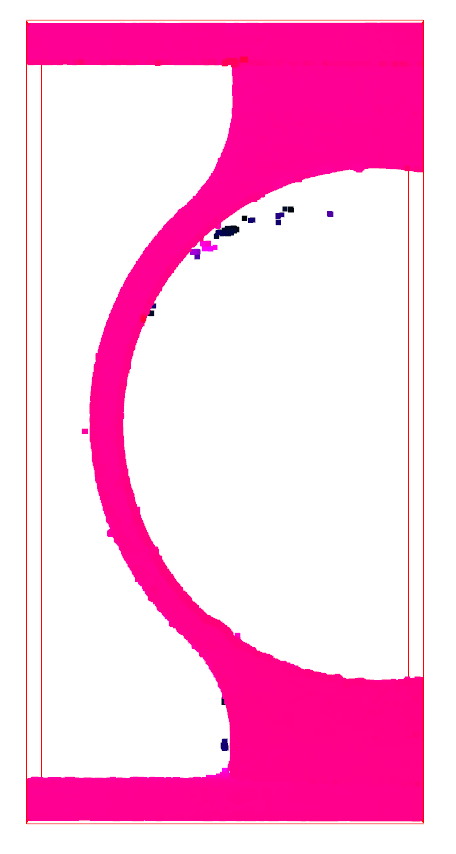
\includegraphics[width=0.2\textwidth]{images/demonstratorbauteil_top.PNG}
    \smallskip\par
    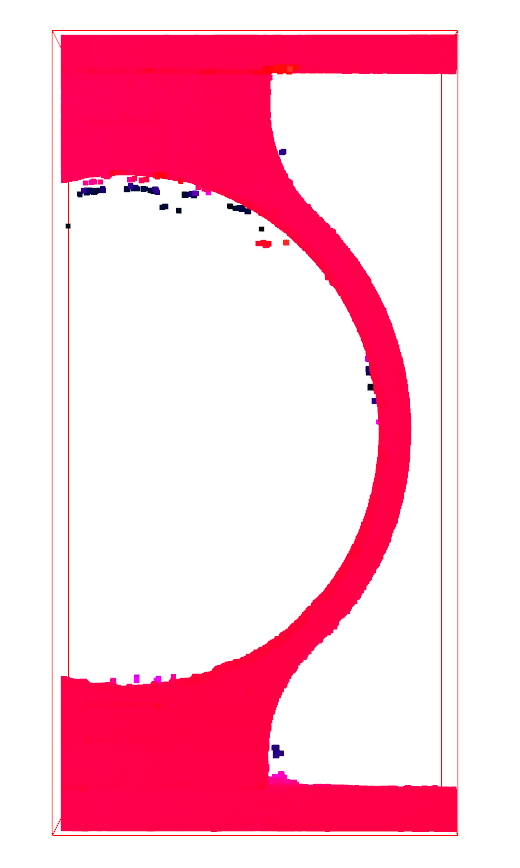
\includegraphics[width=0.2\textwidth]{images/demonstratorbauteil_bottom.PNG}
    \caption{Demonstratorbauteil}
    \label{fig:demonstratorbauteil}
    \vspace{-20pt}
\end{wrapfigure}

Aufgrund der Versprechen dieser Varianten und weil dieser Algorithmus in vielen
Open-Source Bibliotheken schon implementiert ist, war das auch mein erster Ansatz
und ich habe mir Hoffnungen gemacht, dass das Zusammenfügen der Pointclouds 
damit schnell abgehakt ist. 
Dafür habe ich die Methode der Global Registrierung aus der Open3D Bibliothek genutzt
die auf dem Paper von Qian-Yi Zhou, Jaesik Park und Vladlen Koltun basiert. \cite{Zhou.}
Das Globale Registrierung Verfahren wird vor dem ICP-Algorithmus benutzt um eine erste, 
initiale Transformation zu erstellen, die der IPC-Algorithmus im ersten Schritt braucht.

Das Problem bei dieser Methodik und meinem Datensatz ist, das beide Hälften des
Demonstratorbauteils symmetrisch sind. In dem Verfahren wird nicht nur eine Transformation
anhand der X, Y und Z Achsen eingesetzt, sondern auch eine Rotation der Pointcloud.
Wie man in Abbildung \ref{fig:demonstratorbauteil} sehen kann überlappen die beiden Pointclouds 
schon fast zu 100 Prozent, wenn eine Pointcloud um 180 Grad gedreht, und über die andere
gelegt wird. Auf dieses Ergebnis ist auch das Global Registrierungsverfahren gekommen. 
Für unseren Fall ist also ein Verfahren nötig was ausschließlich eine 
Transformation in X und Y Richtung benutzt. Das sind auch die einzigen Achsen, 
in der sich der Scanner bewegt hat.

\subsection*{Wahl des Demonstratorbauteils}

Man könnte sich jetzt hier die Frage stellen, warum das Demonstratorbauteil dann so gewählt 
und entworfen wurde das es symmetrisch ist. In dem ersten Schritt des zusammenfügen ist 
die Bauteilgeometrie zwar hinderlich, dafür profitiert die 
Spannkraftdeformationserkennung von dem initial runden Innenkreis des Bauteils.
Zusätzlich soll das hier zu entwickelnden Verfahren auf viele Bauteilgeometrien 
anwendbar sein und somit nicht durch eine Symmetrie beschränkt werden.

\subsection*{Weitere Verfahren}

Nachdem die globale Registrierung und der ICP-Algorithmus auf den Pointclouds nicht
anwendbar waren musste ein anderes Verfahren her. Aufgrund weniger schon existieren 
Verfahren die eine reine Bewegung auf nur 2 Achsen verwenden habe ich eine Idee 
entworfen, die auf dem ICP-Algorithmus basiert, um 2 Pointclouds zu vergleichen 
und zu verschieben. Hierfür habe ich die Pointclouds in ein zweidimensionales Array
mit den Z-Werten als Inhalt konvertiert. Nun kann die euklidische Distanz der Z-Werte
und jedem X und Y Wert aufsummiert werden. In einem naiven Ansatz kann dann eine 
Pointcloud entlang der Länge und Breite der anderen Pointcloud bewegt werden und für 
jede Transformation die Summe der Distanzen gespeichert werden. Die Idee war das die 
Transformation mit der kleinsten Summe die beste Überlappungen der beiden Pointclouds 
ist. Das hat aber nicht funktioniert. Durch die tatsächliche relativ kleine Überlappung 
ist die Summe der Distanzen nicht bei der korrekten Transformation minimal, 
sondern, wenn die Pointclouds maximal übereinander geschoben sind. Zusätzlich war die 
Verschiebung und Berechnung der zweidimensionalen Arrays rechenintensiv und hat zu 
langen Laufzeiten geführt. Also habe ich dieses Verfahren wieder aufgeben mit einer neuen
Idee:

\subsection*{Pointcloud in Bild konvertieren}
Um Rechenzeit zu sparen und auf viele Funktionen von schon bestehenden 
Bilderkennungs-Bibliotheken zurückgreifen zu können habe ich die Pointclouds in ein
Bild konvertiert. Hierfür wird zuerst in leeres Bild mit den gleichen Maßen einer 
Pointcloud erstellt. Dann wird über alle Punkte der Pointcloud iteriert und jeweils
der Pixel an der X und Y Koordinate des Punktes auf einen Helligkeitswert gesetzt.
Um Rechenzeit und Speicherkapazitäten zu schonen, und weil es für die Berechnung 
ausreichend ist, habe ich mich für 8 Bit Single-Channel Bilder die nur Helligkeitswerte 
abbilden entschieden. Hier kann also jede Pixel einen Wert zwischen 0 und 255 annehmen.
Der entsprechende Wert kann wie folgt berechnet werden:

\begin{wrapfigure}{r}{0.5\textwidth}
    \centering
    $value_p = \frac{Z - min_y}{max_y - min_y} \cdot (max_b - min_b) + min_b$
    \caption{Berechnung Pixelwert}
    \label{calc:brightness}
\end{wrapfigure}
Der resultierende Wert ist die Helligkeit, die dem Pixel zugewiesen wird.
$Z$ ist die Z-Koordinate des Punktes in der Pointcloud. $min_y$ und $max_y$ sind 
die Grenzen der Z-Koordinate, diese werden gebraucht um die Helligkeit relativ 
zu der Höhe zu berechnen. $min_b$ und $max_b$ sind die gewünschten Grenzen der 
Helligkeit. In unserem Fall sind $min_b = 0$ und $max_b = 255$ da ein 8 Bit Bild
verwendet wird.

\begin{wrapfigure}{l}{0.5\textwidth}
    \centering
    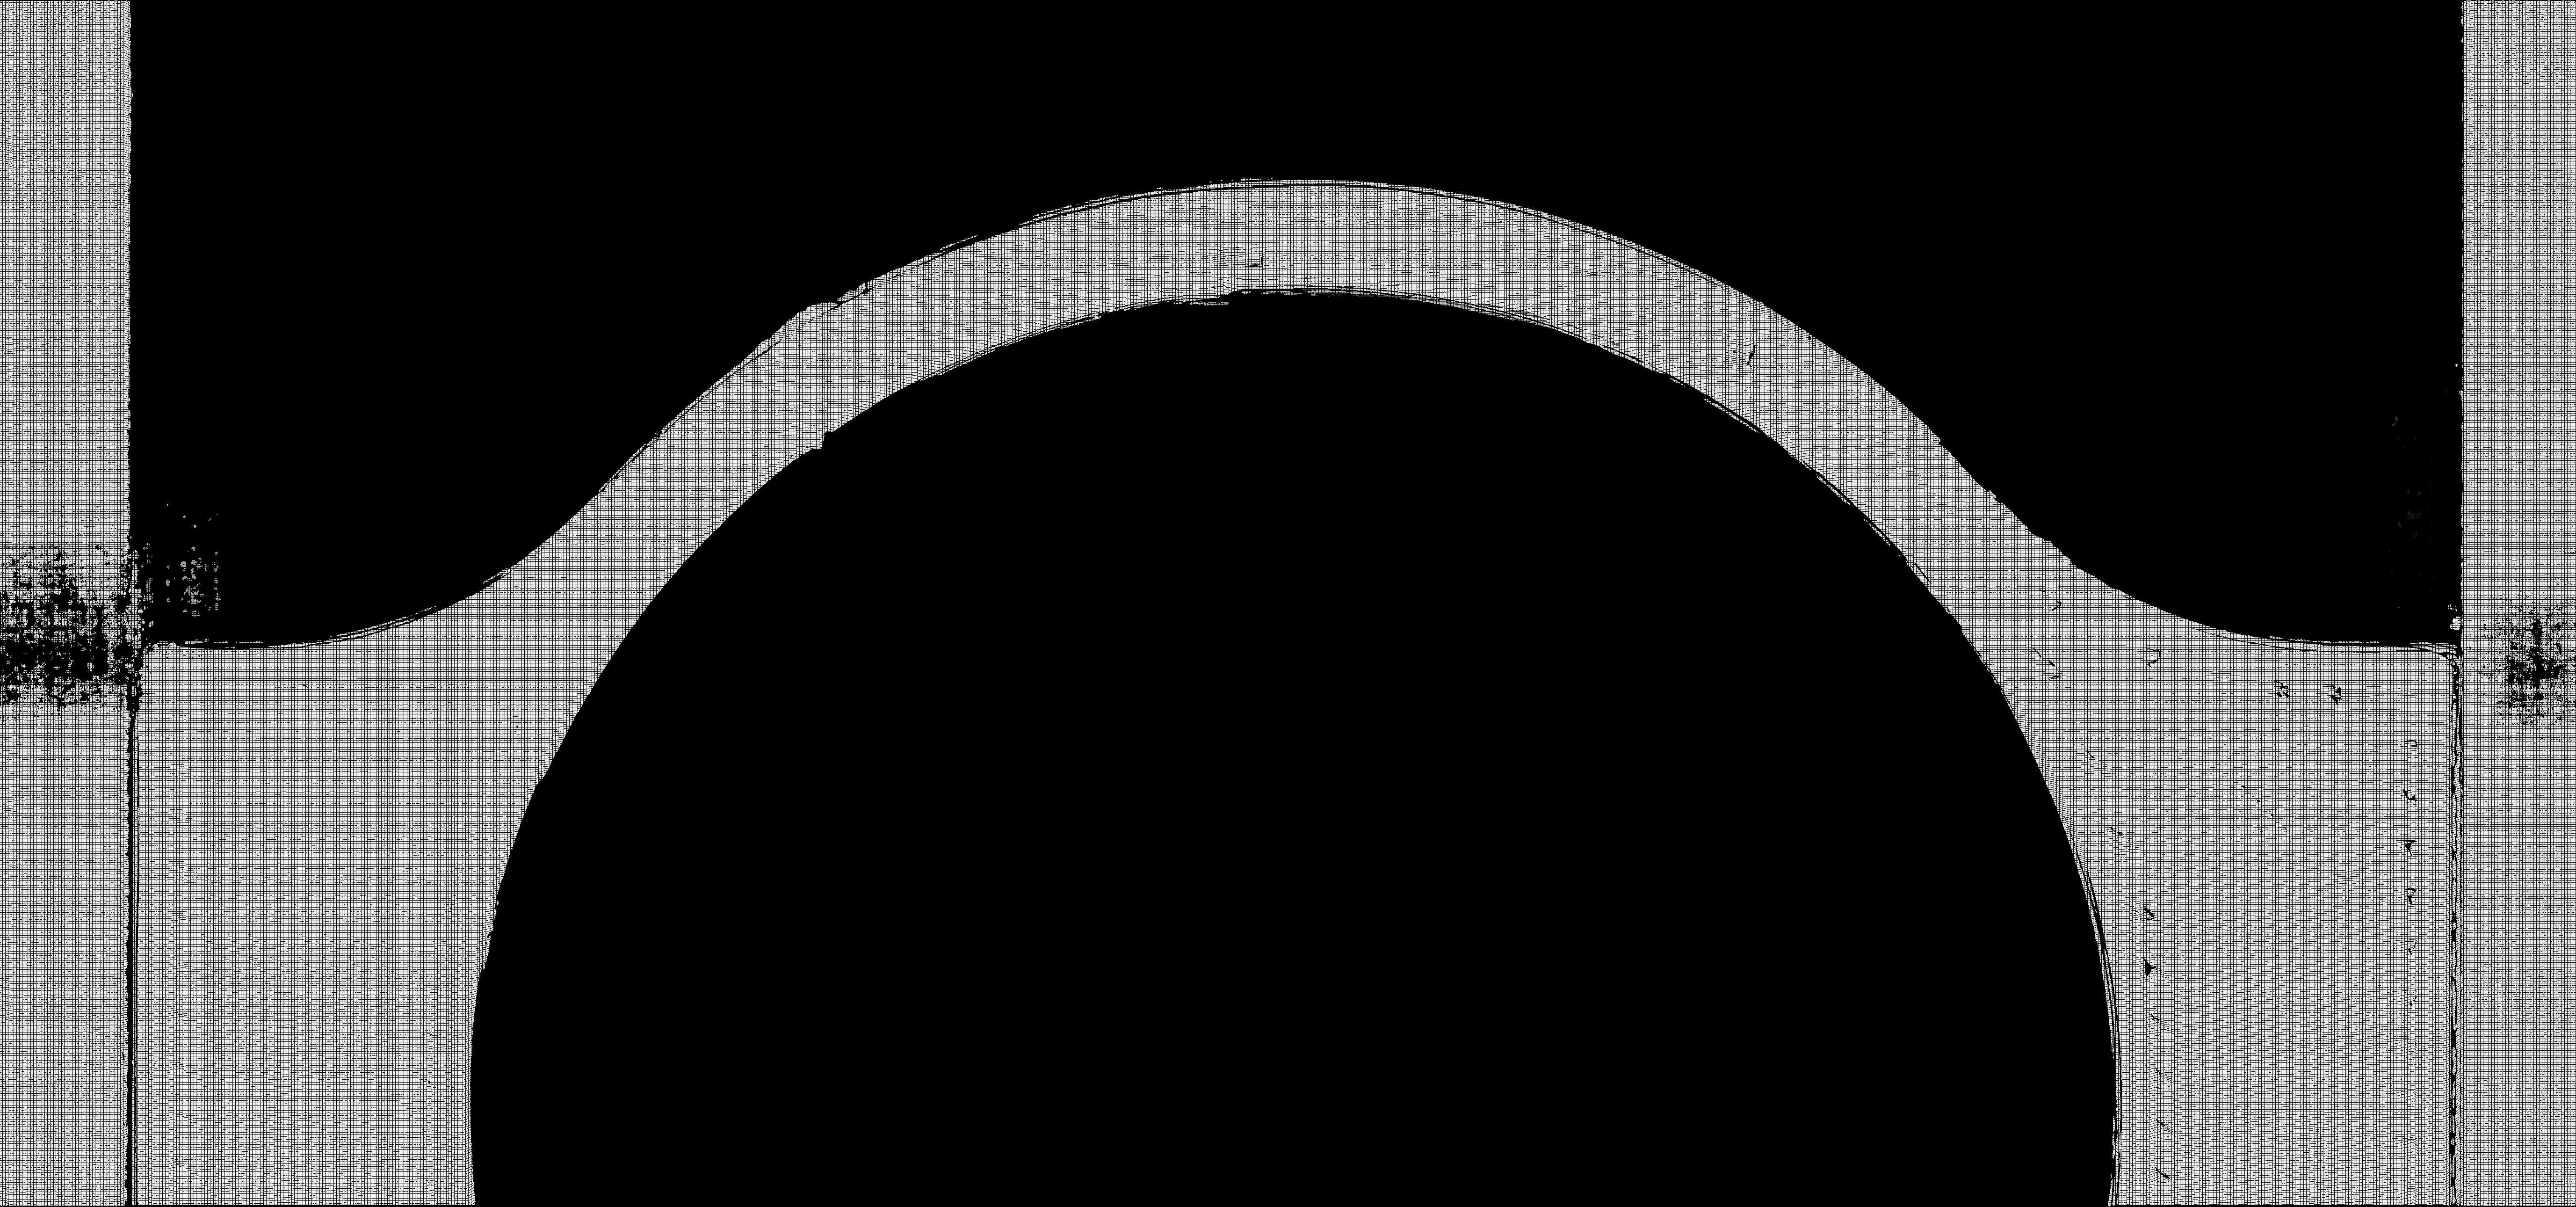
\includegraphics[width=0.5\textwidth]{images/fdm_top_100p.png}
    \includegraphics[width=0.5\textwidth]{images/fdm_top_10p.png}
    \caption{Konvertierung Pointcloud zu Bild}
    \label{fig:image_from_pc}
\end{wrapfigure}

Wie man in Abbildung \ref{fig:image_from_pc} sehen kann, sind kaum Helligkeitsveränderungen
im Bild sichtbar. Das liegt an derselben Problematik, an der der ICP-Algorithmus häufig
scheitert. Reale Datensets wie wir es vorliegen haben sind nicht perfekt, sondern
beinhalten Messfehler und Streuungen. 

Abbildung \ref*{fig:brightness} zeigt die Häufigkeit der gleichen Höhenwerte einer
Pointcloud von dem Demonstratorbauteil als FDM-Druck.
 Auf der y-Achse die relative Häufigkeit.
Die meisten Höhenwerte sind um die 80, sie gehören zu den Punkten, die auf dem 
Demonstratorbauteil liegen, es treten allerdings auch Werte darunter und darüber auf. 
Die in Abbildung \ref*{calc:brightness} vorgestellte Formel benutzt allerdings 
das absolute Minimum und Maximum Werte, 
die Punkte auf dem Bauteil werden also entsprechend wenig
berücksichtigt. Dem kann Abhilfe geschaffen werden, indem Werte, die weniger häufig 
auftreten entfernt werden. Sortiert man alle Höhenwerte nach der Häufigkeit ihres 
auftreten in der Pointcloud und entfernt den n-ten Prozentsatz können Ausreißer 
entfernt werden. Wenn nur die häufigsten 10 Prozent übernommen werden erhält man 
das untere Bild in Abbildung \ref{fig:image_from_pc}

Features auf dem Bauteil können jetzt deutlich besser erkannt werden. Auch zu sehen
sind jetzt die Markierungen auf der linken und Rechten Seite die bei der Registrierung
helfen sollen. Auch schön zu sehen sind die Spuren und Lücken die durch den FDM 
Herstellungsprozess entstehen.

Durch das Filtern der Höheninformationen sind Oberflächenstrukturen nicht nur besser
erkennbar, auch die Ränder treten genauer hervor. Das ist sehr wichtig für das korrekte
zusammenfügen.

Doch wo soll die Grenze gezogen werden, um die Oberfläche möglichst genau zu erkennen,
aber nicht zu viele Höheninformation zu verlieren.

\subsection{Pointcloud filtern}

\begin{wrapfigure}{r}{0.5\textwidth}
    \centering
    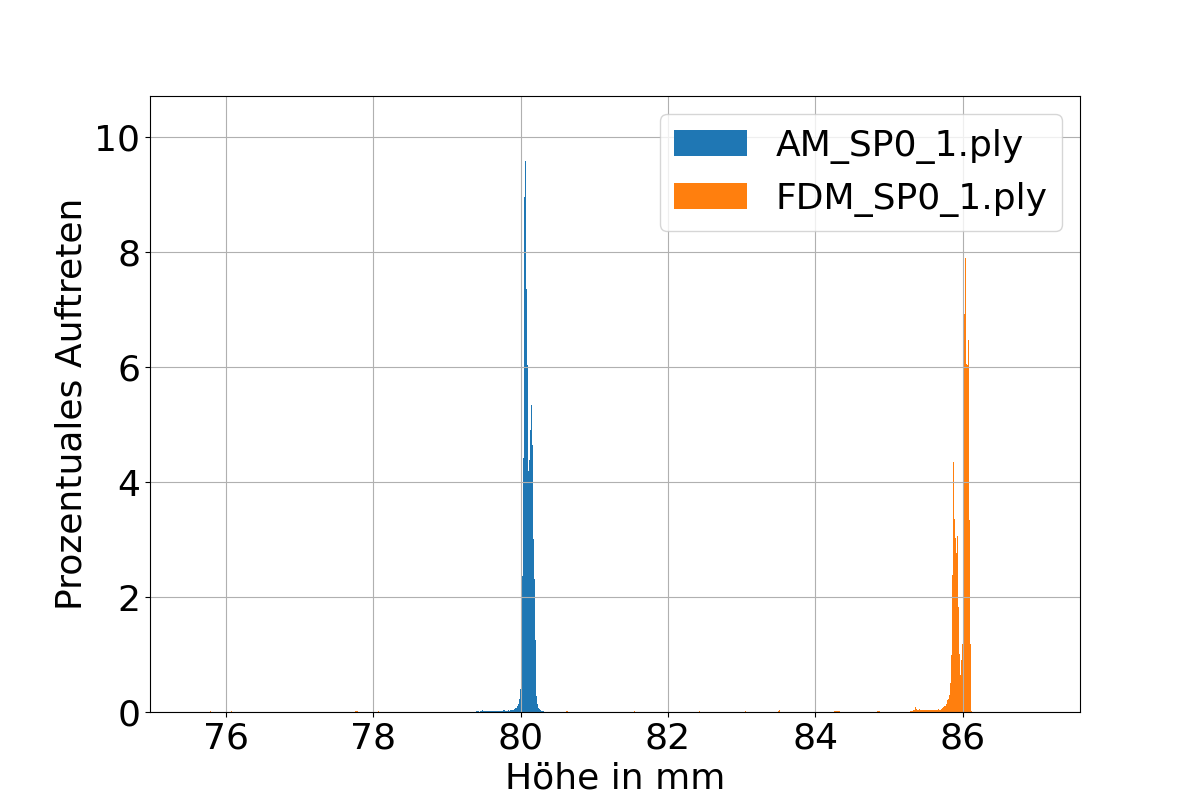
\includegraphics[width=0.5\textwidth]{images/height_occurange.png}
    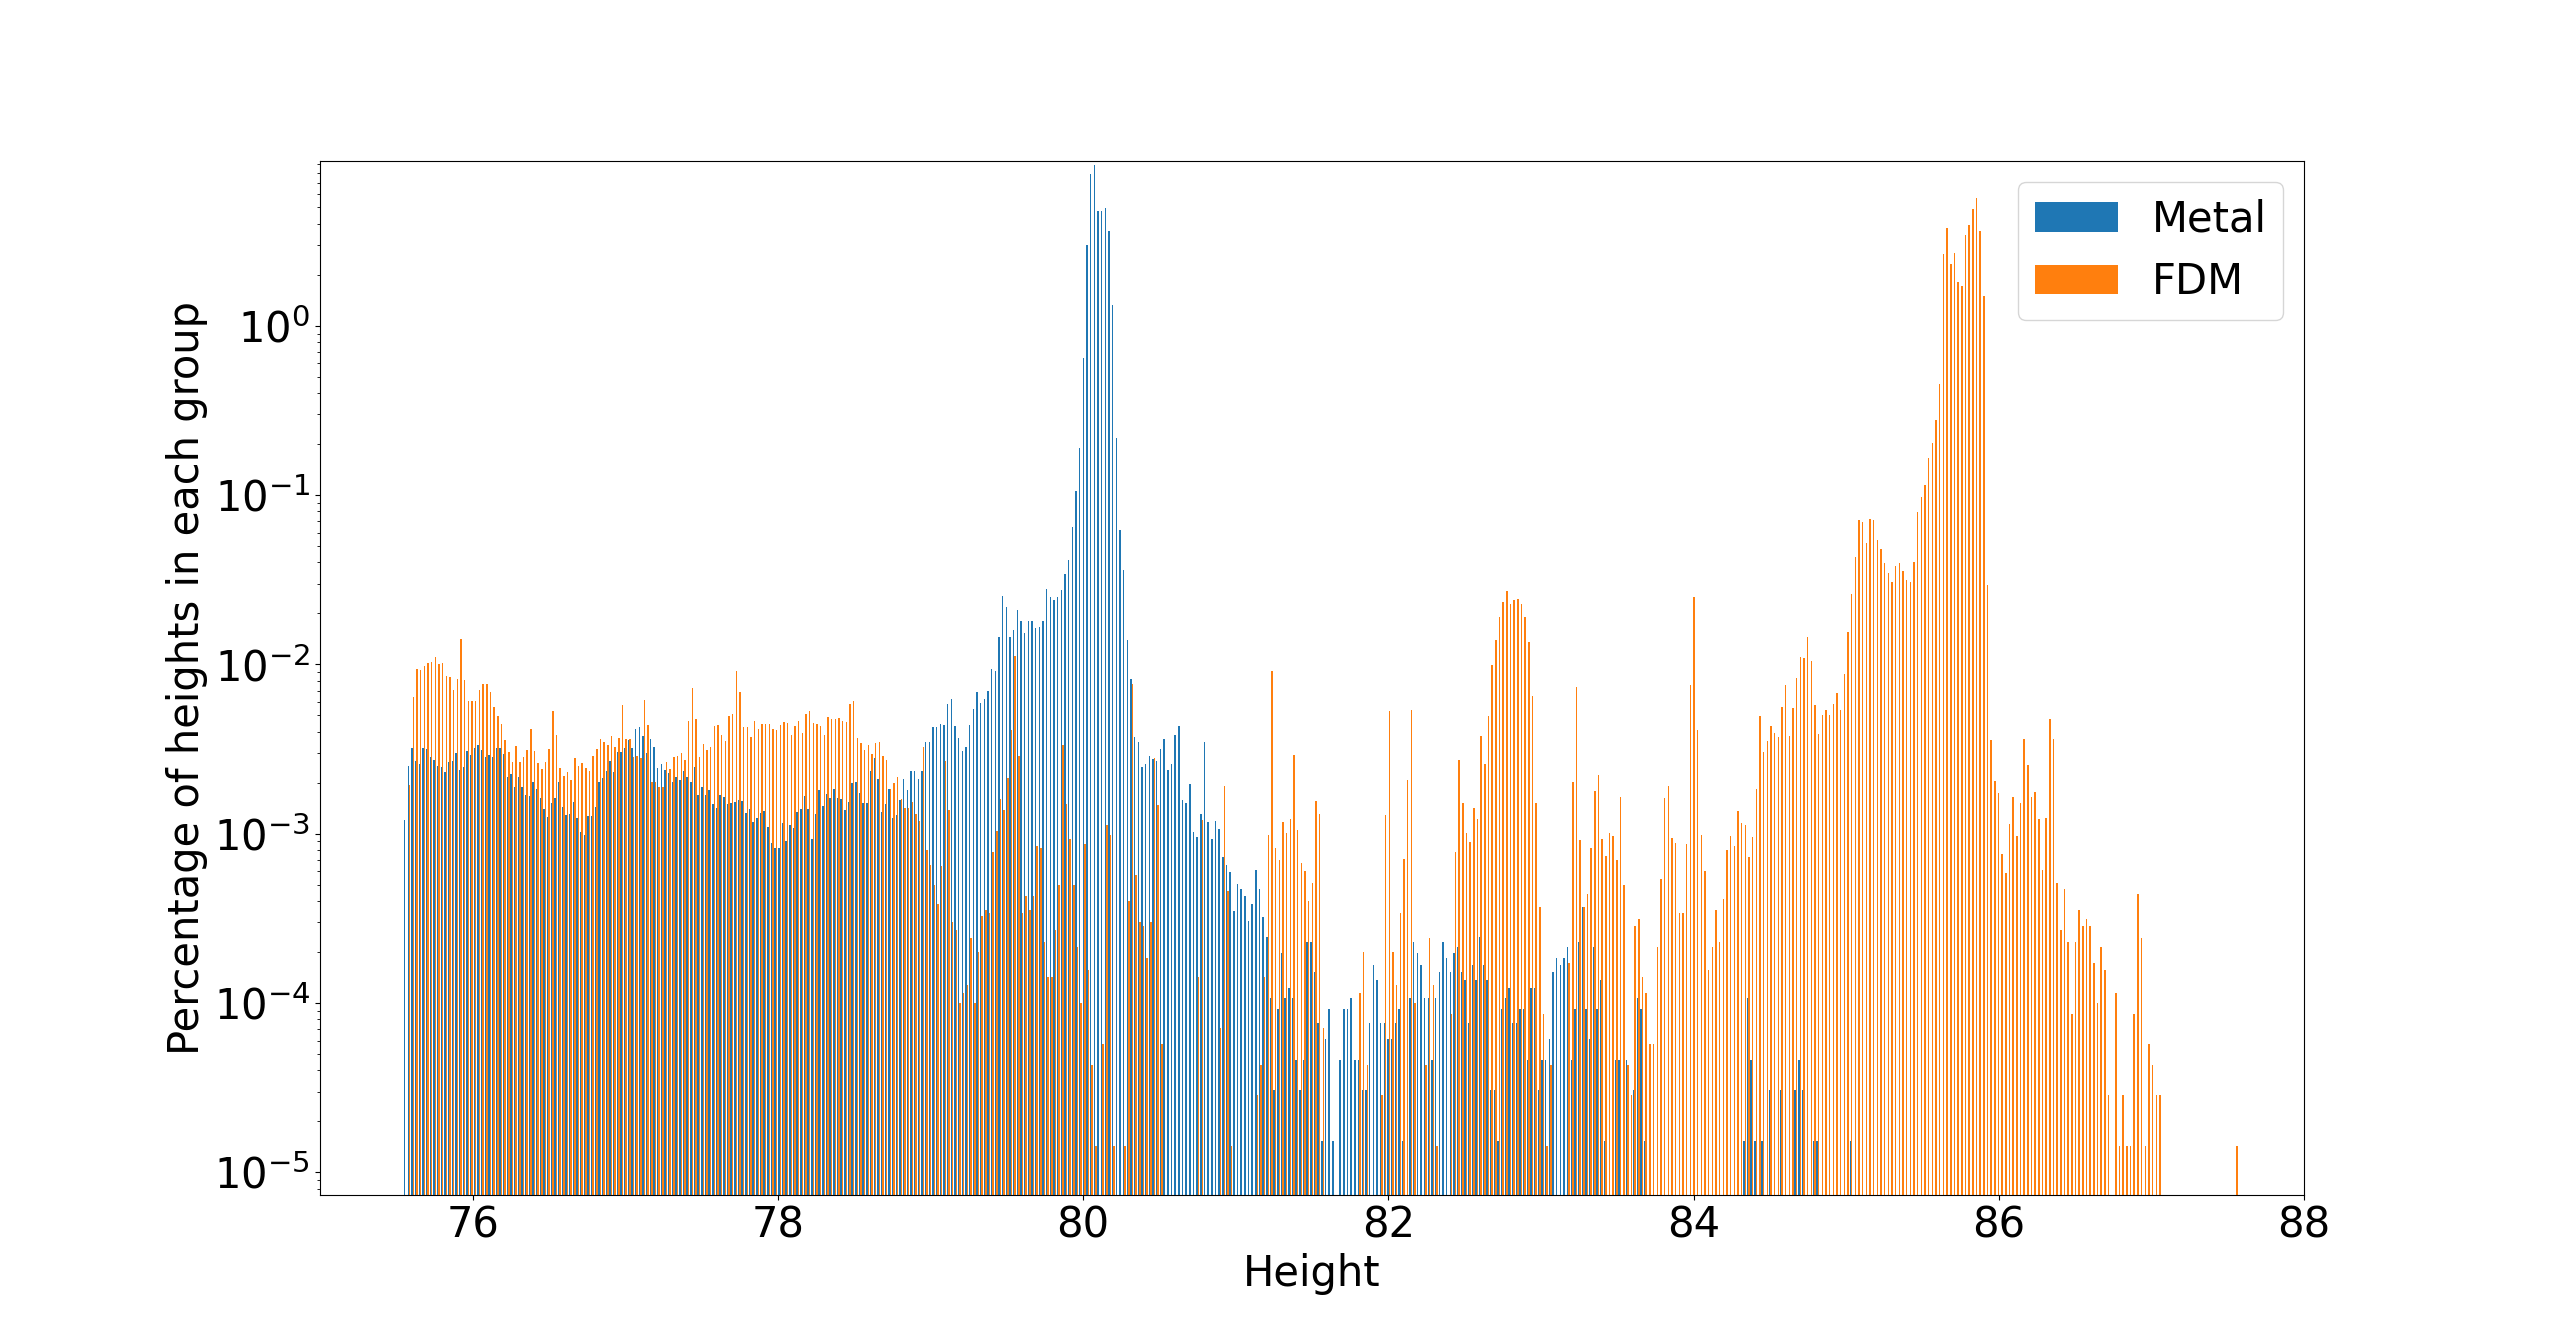
\includegraphics[width=0.5\textwidth]{images/height_occurange_log.png}
    \caption{Auftreten Höhe}
    \label{fig:brightness}
\end{wrapfigure}

Ziel ist das entwickelte Verfahren bei allen gängigen Additiven Fertigungsmethoden
angewendet werden kann, das muss bei der Filterung der Daten berücksichtigt werden
da die Datenverteilung von FDM Bauteilen anders aussieht als bei Metallenen Werkstoffen.
Wie man in Abbildung \ref{fig:brightness} sehen kann streuen nicht alle Pointclouds 
gleich, abhängig von dem Werkstoff des Bauteils werden die Laserstrahlen unterschiedlich
reflektiert und mehr oder weniger Ausreißer sind zu sehen. In dem oberen Histogramm 
sind die Häufigkeiten der Höhenwerte zu sehen, alle Punkte sind in 500 Teile gruppiert.
Unterhalb ist das Histogramm mit dem gleichen Datensatz, aber mit der y-Achse 
logarithmisch
skaliert um kleine Prozente deutlich zu machen die im oberen Diagramm nur schwer oder 
gar nicht sichtbar sind. Man sieht das Metallteil deutlich mehr in beide Richtungen 
streut, während das FDM gedruckte Bauteil weniger nach oben, aber mehr nach unten 
streut. Es muss also eine Filtermethode gewählt werden die für alle Fertigungsverfahren
anwendbar ist und nicht bei einer Methode besser funktioniert wie bei einer 
anderen. Werden zum Beispiel die 10 Prozent häufigst aufkommenden Höhenwerte bei einem
Metallteil benutzt kommt folgendes Bild heraus.

\begin{wrapfigure}{l}{0.4\textwidth}
    \centering
    \includegraphics[width=0.4\textwidth]{images/am_sp0_top_10p.png}
    \caption{Metallteil gefiltert}\label{fig:metall_image}
\end{wrapfigure}

Man sieht vor allem auf der rechten Seite, dass Ränder nicht mehr klar erkennbar sind, 
da sie durch die Filterung Lücken aufweisen. Praxistest haben gezeigt das ein 
ausreichend gut funktionierender Filterwert 50 Prozent ist. Damit werden genug 
Messfehler aus dem Bild genommen aber trotzdem bleiben Oberflächenfeatures und Ränder
sichtbar genug um ein korrektes Zusammenfügen zu gewährleisten.
Dieses Filtern bezieht sich aber nur auf 2 dimensionale Bildinformationen.
Um bei dem Konvertieren noch weniger Punkte die nicht auf dem Bauteil liegen nicht in das Bild zu übernehmen, kann auch noch die Pointcloud gefiltert werden.
Hier kann ein einzelner Punkt relativ zu seinem Nachbarn im 3 dimensionalen Raum betrachtet werden, 
um so Ausreißer zu erkennen. Dafür sind in der Open-Source
Bibliothek 'Open3D' 2 Methoden vorhanden: Radius basiert oder auf Basis von 
statistischen Werten, erste Methode eignet sich gut, wenn die Maße des Objekts bekannt
sind. Hier wird um jeden Punkt eine Kugel gebildet und die Punkte die weniger als 
einen konfigurierbare Menge an Punkte in ihrer Kugel haben werden entfernt. Da 
das hier zu entwickelnde Verfahren sich nicht auf eine Bauteilgeometrie beschränken
ist dieses Verfahren nicht geeignet. Stattdessen wird das andere benutzt. Hier werden
die Punkte entfernt die weiter von ihren benachbarten Punkten entfernt sind als der 
durchschnittliche Abstand der Punkte in der gesamten Pointcloud. Hier kann die Menge der 
benachbarten Punkte die betrachtet werden sollen und ein Limit für den Abstand von der 
Standardabweichung. Umso mehr benachbarte Punkte betrachtet werden, umso mehr Zeit 
braucht die Filterung, aber die Filterung wird auch akkurater. Im Praxistest haben sich
hier 50 Nachbarpunkte bewährt. Mit diesem Wert werden bei Pointclouds in unserem 
Datensatz jeweils ca. 2 Prozent der Punkte entfernt. So kann das resultierende
Bild gut genug umgewandelt werden, um eine erfolgreiche Zusammenführung 
von verschiedenen Bildern zu gewährleisten.
Ein Nachteil bei der Filterung in Abbildung \ref{fig:image_from_pc} links und rechts 
mittig zu sehen. Hier sind schwarze Punkte sichtbar. Diese treten auf, weil der Scanner
hier über dem Bauteil Punkte erkannt hat. Durch das Filtern wurden diese Punkte entfernt
beziehungsweise bei der Konvertierung nicht berücksichtigt. Da diese Punkte dann fehlen
bleiben sie im resultierenden Bild schwarz. Das ist zwar etwas unschön anzuschauen, 
beeinträchtigt das zusammenfügen aber nicht weiter. 

\end{document}